%%%%%%%%%%%%%%%%%%%%%%%%%%%%%%%%%%%%%%%%%
% Short Sectioned Assignment
% LaTeX Template
% Version 1.0 (5/5/12)
%
% This template has been downloaded from:
% http://www.LaTeXTemplates.com
%
% Original author:
% Frits Wenneker (http://www.howtotex.com)
%
% License:
% CC BY-NC-SA 3.0 (http://creativecommons.org/licenses/by-nc-sa/3.0/)
%
%%%%%%%%%%%%%%%%%%%%%%%%%%%%%%%%%%%%%%%%%

%----------------------------------------------------------------------------------------
%	PACKAGES AND OTHER DOCUMENT CONFIGURATIONS
%----------------------------------------------------------------------------------------

\documentclass[paper=a4, fontsize=11pt]{scrartcl} % A4 paper and 11pt font size

\usepackage[T1]{fontenc} % Use 8-bit encoding that has 256 glyphs
\usepackage{fourier} % Use the Adobe Utopia font for the document - comment this line to return to the LaTeX default
\usepackage[english]{babel} % English language/hyphenation
\usepackage{amsmath,amsfonts,amsthm, pgf, tikz} % Math packages
\usetikzlibrary{arrows, automata}
\usepackage{fancyhdr}
\usepackage{lipsum} % Used for inserting dummy 'Lorem ipsum' text into the template

\usepackage{sectsty} % Allows customizing section commands
\allsectionsfont{\centering \normalfont\scshape} % Make all sections centered, the default font and small caps

\usepackage{fancyhdr} % Custom headers and footers
\pagestyle{fancyplain} % Makes all pages in the document conform to the custom headers and footers
\fancyhf{}
\fancyhead[R]{Tyler O. Moses}
\fancyhead[L]{MDA 3105}
\fancyhead[C]{Discrete Mathematics II}
\fancyfoot[L]{} % Empty left footer
\fancyfoot[C]{} % Empty center footer
\fancyfoot[R]{\thepage} % Page numbering for right footer
\renewcommand{\headrulewidth}{0pt} % Remove header underlines
\renewcommand{\footrulewidth}{0pt} % Remove footer underlines
\setlength{\headheight}{13.6pt} % Customize the height of the header

\numberwithin{equation}{section} % Number equations within sections (i.e. 1.1, 1.2, 2.1, 2.2 instead of 1, 2, 3, 4)
\numberwithin{figure}{section} % Number figures within sections (i.e. 1.1, 1.2, 2.1, 2.2 instead of 1, 2, 3, 4)
\numberwithin{table}{section} % Number tables within sections (i.e. 1.1, 1.2, 2.1, 2.2 instead of 1, 2, 3, 4)

\setlength\parindent{0pt} % Removes all indentation from paragraphs - comment this line for an assignment with lots of text

%----------------------------------------------------------------------------------------
%	TITLE SECTION
%----------------------------------------------------------------------------------------

\newcommand{\horrule}[1]{\rule{\linewidth}{#1}} % Create horizontal rule command with 1 argument of height

\title{	
\normalfont \normalsize 
\textsc{Florida State University} \\ [25pt] % Your university, school and/or department name(s)
\horrule{0.5pt} \\[0.4cm] % Thin top horizontal rule
\huge Assignment 1: Relations and Their Properties \\ % The assignment title
\horrule{2pt} \\[0.5cm] % Thick bottom horizontal rule
}

\author{Tyler Moses} % Your name

\date{\normalsize January 18, 2018} % Today's date or a custom date

\begin{document}

\maketitle % Print the title

%----------------------------------------------------------------------------------------
%	PROBLEM 1
%----------------------------------------------------------------------------------------

\section{Exercise}

For the relation: $R = \{(1, 3), (1, 4), (2, 3), (2, 4), (3, 1), (3, 4)\}$ on the set $A=\{1,2,3,4\}$, explain/show whether or not the relation is the following:

(a) reflexive,

(b) symmetric

(c) antisymmetric

(d) transitive

\subsection{Solution}

\textbf{(a) reflexive:} 

Assume that the relation above is reflexive, then $\forall a \in A \implies (a,a) \in R$ however $1 \in A $ and $(1,1) \not\in R$ $\blacksquare$

\textbf{(b) symmetric:} 

If $R$ was symmetric then, $\forall (a,b) \in R \implies (b,a) \in R$, however $(1,4) \in R \land (4,1) \not\in R$ $\blacksquare$

\textbf{(c) antisymmetric:}

If $R$ was antisymmetric, then $\forall x \forall y  [((x,y) \in R \land (y,x)) \in R \implies (x = y)]$, however $(1,3) \in R \land (3,1) \in R \land (1 \neq 3)$  $\blacksquare$

\textbf{(d) transitive:}

If $R$ was transitive, then $\forall x \forall y \forall z [(x,y) \in R \land (y,z) \in R \implies (x,z) \in R]$, however $(1,3) \in R \land (3,1) \in R \land (1,1) \not\in R$ $\blacksquare$

%----------------------------------------------------------------------------------------
%	PROBLEM 2
%----------------------------------------------------------------------------------------

\section{Exercise}

Let the sets be relations on the real numbers: $R_1=\{(a,b) \in \mathbb{R}^2 \vert a \geq b \}$, the "greater than or equal to" relation, and let $R_2 = \{ (a,b) \in \mathbb{R}^2 \vert a \neq b \}$, the "unequal to" relation. Find:

(a) $R_1 \cap R_2$

(b) $R_1 - R_2$

(c) $R_1 \oplus R_2$

\subsection{Solution}

\textbf{(a) $R_1 \cap R_2$:} 

Let $R = R_1 \cap R_2$, then by definition $$R = \{ (a,b) \in \mathbb{R}^2 \vert (a \geq b)  \land (a \neq b) \} \implies R = \{ (a,b) \in \mathbb{R}^2 \vert (a > b) \} \blacksquare$$ 

\textbf{(b) $R_1 - R_2$:} 

Let $R = R_1 - R_2$, then by definition: $$R = R_1 \cap \overline{R_2} = \{ (a,b) \in \mathbb{R}^2 \vert (a \geq b) \land \neg(a \neq b) \} = \{ (a,b) \in \mathbb{R}^2 \vert (a \geq b) \land (a = b) \}  = \{ (a,b) \in \mathbb{R}^2 \vert (a = b) \} \blacksquare$$

\textbf{(c) $R_1 \oplus R_2$:}

Let $R = R_1 \oplus R_2$, then: $$R = (R_1 - R_2) \cup (R_2 - R_1)$$ where, $$(R_2 - R_1) = R_2 \cap \overline{R_1} = \{ (a,b) \in \mathbb{R}^2 \vert (a \neq b) \land \neg (a \geq b) \} = \{ (a,b) \in \mathbb{R}^2 \vert (a \neq b) \land (a < b) \} = \{ (a,b) \in \mathbb{R}^2 \vert (a < b) \} $$ and $$R_1 - R_2 =  \{ (a,b) \in \mathbb{R}^2 \vert (a = b) \}$$ from the previous example. Therefore: $$R = \{ (a,b) \in \mathbb{R}^2 \vert (a = b) \lor (a < b) \} = \{ (a,b) \in \mathbb{R}^2 \vert (a \leq b) \} \blacksquare$$

%----------------------------------------------------------------------------------------
%	PROBLEM 3
%----------------------------------------------------------------------------------------

\section{Exercise}

(a) How many \textbf{binary} relations are there on the set $\{a,b,c\}$?

(b) If $R = \{(1,1),(1,2),(2,4),(3,1),(3,0)\}$, $S=\{(1,2),(2,0),(3,1),(0,0),(4,3)\}$ find $R \circ S$

\subsection{Solution}

\textbf{(a) How many \textbf{binary} relations are there on the set $\{a,b,c\}$?} 

By definition a binary operation is a subset of the cartesian product of $A$, therefore we have $2^n$ where $n = \vert A X A \vert = \vert A \vert x \vert A \vert = 3 x 3 = 9$ therefore $2^9 \blacksquare$ 

\textbf{(b) If $R = \{(1,1),(1,2),(2,4),(3,1),(3,0)\}$, $S=\{(1,2),(2,0),(3,1),(0,0),(4,3)\}$ find $R \circ S$} 

By definition, $$R \circ S = \{ (a,c) \vert (a,b) \in R \land (b,c) \in S (\exists b) \}$$ or $$R \circ S  = \{ (1,2), (1,0), (2,3), (3,2), (3,0) \}$$

%----------------------------------------------------------------------------------------
%	PROBLEM 4
%----------------------------------------------------------------------------------------

\section{Exercise}

R is the relation represented by the matrix $M_R = 
\begin{bmatrix}
1 & 0 & 0 \\
1 & 1 & 1 \\
0 & 1 & 0
\end{bmatrix}
$, find the matrix for:

(a) $R^{-1}$

(b) $\overline{R}$

(c) $R \circ R$

\subsection{Solution}

\textbf{(a)} $R^{-1} = \begin{bmatrix}
1 & 1 & 0 \\
0 & 1 & 1 \\
0 & 1 & 0
\end{bmatrix}
$

\textbf{(b)} $\overline{R} = \begin{bmatrix} 
0 & 1 & 1 \\
0 & 0 & 0 \\
1 & 0 & 1
\end{bmatrix}$

\textbf{(c)} $R \circ R = \begin{bmatrix}
1 & 0 & 0 \\
1 & 1 & 1 \\
1 & 1 & 1
\end{bmatrix}$

%----------------------------------------------------------------------------------------
%	PROBLEM 5
%----------------------------------------------------------------------------------------

\section{Exercise}

(a) The relation $R$ is on $\{ 1, 2, 3 \}$. Represent the relation $$R = \{ (1,1), (2,1), (2,2), (2,3), (3,2) \}$$ with a matrix.

(b) By looking at the matrix, is the relation $R$ reflexive? Why or why not?

(c) Draw the directed graph that represents the relation R.

\subsection{Solution}

\textbf{(a) Represent the above relation as a matrix.}

$$M_R = \begin{bmatrix}
1 & 0 & 0 \\
1 & 1 & 1 \\
0 & 1 & 0
\end{bmatrix}$$

\textbf{(b) Does this matrix represent a reflexive relation?}

No, $\exists i \vert M_{i,i} \neq 1$ aka $M_{3,3} = 0$.

\textbf{(c) Draw the directed graph that represents the relation R.}
$$
  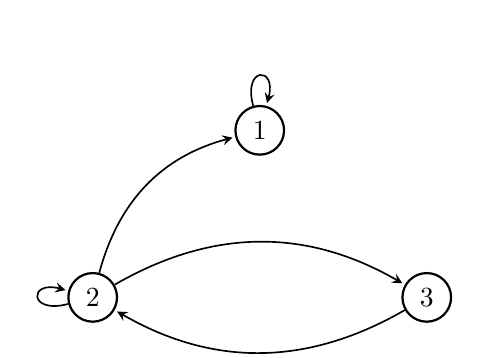
\begin{tikzpicture}[
            > = stealth, % arrow head style
            shorten > = 1pt, % don't touch arrow head to node
            auto,
            node distance = 3cm, % distance between nodes
            semithick % line style
        ]

        \tikzstyle{every state}=[
            draw = black,
            thick,
            fill = white,
            minimum size = 4mm
        ]

        \node[state] (1) {$1$};
        \node[state] (2) [below left of=1] {$2$};
        \node[state] (3) [below right of=1] {$3$};
        %\node[state] (v1) [above right of=s] {$v_1$};
        %\node[state] (v2) [right of=s] {$v_2$};
        %\node[state] (v3) [below right of=s] {$v_2$};
        %\node[state] (t) [right of=v2] {$t$};

	\path[->] (1)  [loop above] edge (1);
	\path[->] (2) [bend left] edge (1);
	\path[->] (2) [loop left] edge (2);
	\path[->] (2) edge [bend left] (3);
	\path[->] (3) edge [bend left] (2);
        %\path[->] (s) edge node {18} (v1);
        %\path[->] (s) edge node {1} (v2);
        %\path[->] (s) edge node {1} (v3);
        %\path[->] (v2) edge node {2} (v1);
        %\path[->] (v3) edge node {1} (v2);
        %\path[->] (v1) edge node {20} (t);

        %\draw[red, dashed] (1, 2) -- (1, -2);
    \end{tikzpicture}
$$
%----------------------------------------------------------------------------------------
%	END DOCUMENT
%----------------------------------------------------------------------------------------

\end{document}